% tikzpic.tex
\documentclass[crop,tikz]{standalone}% 'crop' is the default for v1.0, before it was 'preview'
%\usetikzlibrary{...}% tikz package already loaded by 'tikz' option

\usepackage{amsmath}
\usepackage{mathtools}
\usepackage{amssymb,amsthm}
\usepackage[normalem]{ulem}
\usepackage{bm}
\usepackage{pgfplots}

\usepackage{tikz}
\usetikzlibrary{positioning, calc, chains}



\begin{document}



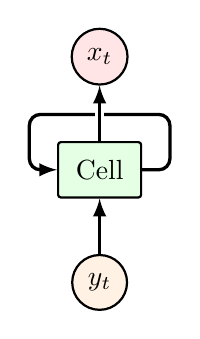
\begin{tikzpicture}[
	cell/.style={rectangle, rounded corners=1pt, draw,thick,align=center, fill=green!10,
		minimum width=30pt, minimum height=20pt},
	item/.style={circle,draw,thick,align=center},
	itemc/.style={cell,on chain,join}
	]
	\node[cell] (AL) {Cell};
	\path (AL.west) ++ (-1em,2em) coordinate (aux);
	\draw[very thick,-latex,rounded corners] (AL.east) -| ++ (1em,2em) -- (aux) 
	|- (AL.west);

	\draw[white,line width=0.8ex] (AL.north) -- ++ (0,1.9em);
	\draw[very thick,-latex] (AL.north) -- ++ (0,2em)
	node[above,item,fill=red!10] {$x_t$};
	\draw[very thick,latex-] (AL.south) -- ++ (0,-2em)
	node[below,item,fill=orange!10] {$y_t$};
        
         
\end{tikzpicture}

\end{document}